\documentclass[11pt,a4paper]{article}
\usepackage[T1]{fontenc}\usepackage[utf8]{inputenc}
\usepackage{lmodern,microtype,amsmath,amssymb,amsthm,mathtools}
\usepackage{booktabs,longtable,array,enumitem,xcolor,geometry,fancyhdr,hyperref,graphicx}
\geometry{margin=21mm}
\hypersetup{colorlinks=true,linkcolor=blue!55!black,urlcolor=blue,
 pdftitle={FIN ST2262--ST2351: Composition, Automorphism and Fractal Fixed-Point Tests},
 pdfauthor={Krzysztof Żuchowski}}
\pagestyle{fancy}\fancyhf{}
\fancyhead[L]{FIN ST2262--ST2351}\fancyhead[R]{Release 11.09}
\fancyfoot[C]{\thepage}\setlength{\headheight}{14pt}
\newtheorem{theorem}{Theorem}\newtheorem{proposition}{Proposition}
\newcommand{\status}[1]{\textsf{[#1]}}

\begin{document}
\begin{titlepage}\centering\vspace*{13mm}
{\Huge\bfseries Composition, Automorphism and\par}\vspace{2mm}
{\Huge\bfseries Fractal Fixed-Point Tests\par}\vspace{5mm}
{\LARGE The Identity-or-Erasure Theorem and\par}\vspace{2mm}
{\LARGE the Minimal Ternary Instrument\par}\vspace{10mm}
{\Large FIN ST2262--ST2351\par}\vspace{8mm}
{\Large Krzysztof \.Zuchowski\par}
{\normalsize Independent Researcher --- Fractal Information Theory Project\par}
{\normalsize ORCID: 0009-0002-0909-3613\par}\vspace{8mm}
{\large Six adaptive research rounds --- 90 programmes\par}
{\large Release 11.09 --- 1 September 2026\par}
\vfill
\begin{minipage}{.88\textwidth}\small
Release 11.08 found the strict loop-product flag lift but left two possible
routes to uniqueness: separate edge linearity plus face universality, or a
fractal refinement principle selecting the Hodge exponent.  This report tests
both routes, proves an identity-or-erasure theorem for exact finite
self-similarity, and constructs the smallest instrument capable of observing
irreducible three-point information.
\end{minipage}\vfill
{\small English mathematical research report. CC BY 4.0.}
\end{titlepage}

\begin{abstract}
The strict loop-product field
\[
 \tau_{ijk}=W_{ij}W_{jk}W_{ki}
\]
supports the positive Hodge family
\[
 h_f(p)=\frac{\tau_f^p}{\langle\tau^p\rangle},\qquad p>0.
\]
Release 11.09 asks whether the exponent \(p=1\) can be forced without inserting
new physics.

The first route fails.  Dirichlet energy is exactly additive under parallel
addition of edge conductances, but this does not determine how three edge
weights compose into one face weight.  The product is separately additive,
whereas the geometric mean, harmonic mean and minimum are equally local,
positive, symmetric and support-zero but are not separately additive.
Separate edge linearity is therefore an additional face-lift axiom.

The second premise, face universality, also fails.  All six strict
cyclic-distance weights are distinct.  The maximum-weight edges form
\(C_{12}\), so every weighted automorphism belongs to
\(\operatorname{Aut}(C_{12})=D_{12}\); conversely \(D_{12}\) preserves every
weight.  Hence
\[
 \operatorname{Aut}(W)=D_{12}.
\]
This group has twelve triangle orbits, all distinguished by the strict loop
product.  Equivariance permits twelve face coefficients rather than one.

A stronger conditional result does exist.  For a positive profile define
\[
 T_p(x)=\frac{x^p}{\langle x^p\rangle}.
\]
Then
\[
 T_p\circ T_q=T_{pq}.
\]
For any nonconstant positive profile, scale-stationary path independence
\(T_p^2x=T_px\) implies \(p^2=p\).  Thus only \(p=0\) and \(p=1\) survive.
The first erases the profile to uniformity; the second is the identity.  Even
self-similarity up to a permutation of the twelve orbits forces \(p=1\).
Consequently exact finite power self-similarity supplies no nontrivial
compression dynamics.

Ordinary coassociativity is weaker and leaves a continuous rate:
\(p(t)=e^{-ct}\), or one exponent per refinement level.  This agrees with the
existing FIN refinement theorems, which leave unsourced vertical rates.  The
conditional \(p=1\) theorem therefore cannot be promoted to strict FIN.

Finally, the minimal observable for the hidden-synergy family is
\(Y=x_1x_2x_3\).  Pair-only Fisher information is zero, whereas parity has
\[
 I(\varepsilon)=\frac1{1-\varepsilon^2}.
\]
The estimator \(\widehat\varepsilon=\overline Y\) is efficient.  Nineteen
events suffice under a Hoeffding bound to determine the sign for
\(|\varepsilon|\geq0.75\) with declared error \(0.01\).  A minimal
non-Gaussian model is
\[
 p_\theta(x)=\frac{e^{\theta x_1x_2x_3}}{8\cosh\theta},
 \qquad \varepsilon=\tanh\theta.
\]
It explicitly adds the absent three-body statistic and source parameter.

The gate contains seven valid mathematical constructions, three strict-source
rows, and zero physical rows.  The pair/refinement route is a bounded no-go on
current artifacts.  A future result can change the verdict only by exporting a
strict non-Gaussian three-body state law with nonzero connected cumulant, fixed
polarity and coherent refinement transport.
\end{abstract}

\tableofcontents\newpage

\section{Input discipline}

The report retains the strict/legacy split.  It uses the strict positive
Dirichlet conductances \(W\) in
\[
 A=sI-W,\qquad
 \langle f,Af\rangle=\frac12\sum_{x,y}W_{xy}|f_x-f_y|^2.
\]
No legacy physical role is transferred.  The raw legacy loop products have
both signs, so noninteger powers are not real without an additional absolute
value, sign sector or completion rule.

The question is not whether \(p=1\) is an elegant convention.  It is whether
the current mathematics makes every alternative impossible.

\section{Round I: ST2262--ST2276 --- separate linearity}

For fixed \(f\), the Dirichlet energy is linear in the edge conductance matrix:
\[
 E_{W+W'}(f)=E_W(f)+E_{W'}(f).
\]
The finite replay gives residual zero.  This is an edge-level statement.

\begin{theorem}[conditional separate-additivity theorem]
Let \(F(a,b,c)\) be continuous, vanish when any argument vanishes, and be
additive independently in each positive argument.  Then
\[
 F(a,b,c)=\kappa abc.
\]
\end{theorem}

Thus independent preservation of parallel addition selects the loop product.
The key point is that FIN has not exported this preservation law for the
edge-to-face lift.

The following target-free counterrules satisfy locality, positivity, symmetry
and support-zero:
\[
 (abc)^{1/3},\qquad
 \frac3{a^{-1}+b^{-1}+c^{-1}},\qquad
 \min(a,b,c).
\]
On a fixed strict weight tuple their separate-additivity defects are,
respectively,
\[
 -0.0785221321,\quad -0.0785966273,\quad -0.0470291687,
\]
while the product residual is numerical zero.

There is also a homogeneity ambiguity.  The product has total degree three;
the three counterrules have degree one.  Current strict data do not assign a
physical dimension or scaling degree to a face stiffness.  Edge-energy
linearity therefore does not force face multilinearity.

\section{Round II: ST2277--ST2291 --- face universality}

The six strict distance weights are distinct, with minimum pair separation
\(0.0130604060\).  Distance-one edges have the unique maximum and form the
cycle \(C_{12}\).

\begin{theorem}[weighted automorphism group]
\[
 \operatorname{Aut}(W)=D_{12}.
\]
\end{theorem}
\begin{proof}
Every weighted automorphism preserves the unique maximum-weight subgraph,
which is \(C_{12}\), so it belongs to
\(\operatorname{Aut}(C_{12})=D_{12}\).  Conversely every dihedral symmetry
preserves cyclic distance and all six weights.
\end{proof}

The direct finite conjugation residual is zero for all 24 elements.  A
non-dihedral transposition gives residual \(0.9178297\), and multiplication by
the unit \(5\in\mathbb Z_{12}\) also fails because it permutes unequal distance
weights.

There are twelve \(D_{12}\)-orbits of triangles.  The twelve loop-product
values are distinct; their smallest separation is
\(2.5670\times10^{-7}\).  The strict data therefore retain, rather than erase,
the orbit labels.

Full \(S_{12}\) symmetry would make every triangle equivalent, but it is not a
symmetry of the strict weighted graph.  One universal formula on all weighted
graphs is a valid category-level axiom, not an internal consequence of
\(\operatorname{Aut}(W)\).

\section{Round III: ST2292--ST2306 --- conditional exponent theorem}

\begin{theorem}[continuous multiplicative valuations]
Every continuous positive solution of
\[
 g(xy)=g(x)g(y)
\]
has \(g(x)=x^p\).  Monotonicity gives \(p\geq0\).
\end{theorem}

After mean normalization,
\[
 T_p(T_q(x))=T_{pq}(x).
\]
The strict orbit-vector replay gives residual \(3.55\times10^{-15}\).

\begin{theorem}[idempotent exponent classification]
Let \(x\) be positive and nonconstant.  If
\[
 T_p(T_p(x))=T_p(x),
\]
then \(p\in\{0,1\}\).
\end{theorem}
\begin{proof}
Choose \(x_i\neq x_j\).  Ratios remove normalization:
\[
 \left(\frac{x_i}{x_j}\right)^{p^2}
 =\left(\frac{x_i}{x_j}\right)^p.
\]
Since the base ratio is positive and not one, \(p^2=p\).
\end{proof}

The \(p=0\) branch maps everything to the uniform profile and erases all orbit
information.  The \(p=1\) branch preserves information but is the identity.

Therefore \(p=1\) follows only from the conjunction:
\begin{enumerate}
\item positive multiplicative valuation;
\item a nonconstant profile;
\item scale-stationary path independence/idempotence;
\item exclusion of total erasure.
\end{enumerate}
The third premise is stronger than ordinary coassociativity and is not a
strict FIN theorem.

Without it, the continuous semigroup
\[
 p(t)=e^{-ct},\qquad c\geq0,
\]
satisfies \(p(t+s)=p(t)p(s)\) for every rate \(c\).  A rate modulus survives.

\section{Round IV: ST2307--ST2321 --- exact self-similarity}

Let \(x\) be the normalized vector of twelve strict loop-product orbit values
and define centered log coordinates
\[
 y_i=\log x_i-\frac1{12}\sum_j\log x_j.
\]
Then \(T_p\) acts as \(y\mapsto py\).

\begin{theorem}[permuted self-similarity no-go]
For a nonconstant positive \(x\), if
\[
 T_p(x)=Px
\]
for a permutation matrix \(P\) and \(p>0\), then \(p=1\).
\end{theorem}
\begin{proof}
In centered log coordinates, \(py=Py\).  Since a permutation is orthogonal,
\[
 p\|y\|=\|Py\|=\|y\|.
\]
Nonconstancy gives \(\|y\|>0\), hence \(p=1\).
\end{proof}

For \(0<p<1\), normalized power refinement increases entropy and moves the
finite profile toward uniformity.  For \(p>1\), it lowers entropy and sharpens
the largest orbit.  Neither gives an exact nonconstant fixed shape.

The numerical idempotence residuals on the strict profile are
\[
\begin{array}{c|ccccc}
p&0&0.5&1&1.8&2\\ \hline
\|T_p^2x-T_px\|_\infty&0&2.43165&0&0.625304&0.467324.
\end{array}
\]

One may preserve ordinary path composition with level-dependent exponents
\(p_n\), whose cumulative exponent is \(\prod_n p_n\).  This is exactly the
escape already seen in FIN: one refinement rate or vertical mode per level.
It is coherent but not predictive.

\begin{quote}
Exact finite self-similarity selects identity or erasure.  Nontrivial fractal
evolution requires new level-dependent data.
\end{quote}

\section{Round V: ST2322--ST2336 --- minimal ternary instrument}

For
\[
 p_\varepsilon(x)=\frac18(1+\varepsilon x_1x_2x_3),
\]
the minimal distinguishing observable is
\[
 Y=x_1x_2x_3.
\]
Binary-cube character orthogonality proves that \(Y\) cannot be represented as
a sum of one- and two-body functions.  Hence interaction order three is
minimal.

All pair marginals are independent of \(\varepsilon\), so every pair-only
instrument has Fisher information zero.  In contrast,
\[
 \Pr(Y=y)=\frac{1+\varepsilon y}{2},\qquad y=\pm1,
\]
and
\[
 I(\varepsilon)=\frac1{1-\varepsilon^2}.
\]
The estimator
\[
 \widehat\varepsilon=\frac1n\sum_{r=1}^nY_r
\]
is unbiased with variance
\[
 \operatorname{Var}(\widehat\varepsilon)
 =\frac{1-\varepsilon^2}{n},
\]
which reaches the Cram\'er--Rao bound.

For \(\varepsilon_0=0.75\) and declared error \(\delta=0.01\), the two-sided
Hoeffding bound gives
\[
 n\geq\frac{2\log(2/\delta)}{\varepsilon_0^2},
\]
so \(n=19\) events suffice.

The minimal exponential family carrying this statistic is
\[
 p_\theta(x)
 =\frac{\exp(\theta x_1x_2x_3)}{8\cosh\theta},
 \qquad\varepsilon=\tanh\theta.
\]
The likelihood flow
\[
 \dot\theta=\varepsilon_*- \tanh\theta
\]
converges to \(\theta=\operatorname{artanh}\varepsilon_*\) for a supplied
target.  At \(\varepsilon_*=0,\theta(0)=0\), it remains zero.  The model
therefore makes the missing ingredient explicit rather than deriving it.

A Gibbs realization \(H=-Jx_1x_2x_3\) has \(\theta=\beta J\), but \(J,\beta\),
the sign, the preparation and the apparatus are new inputs.

\section{Round VI: ST2337--ST2351 --- synthesis}

\begin{figure}[ht]
\centering
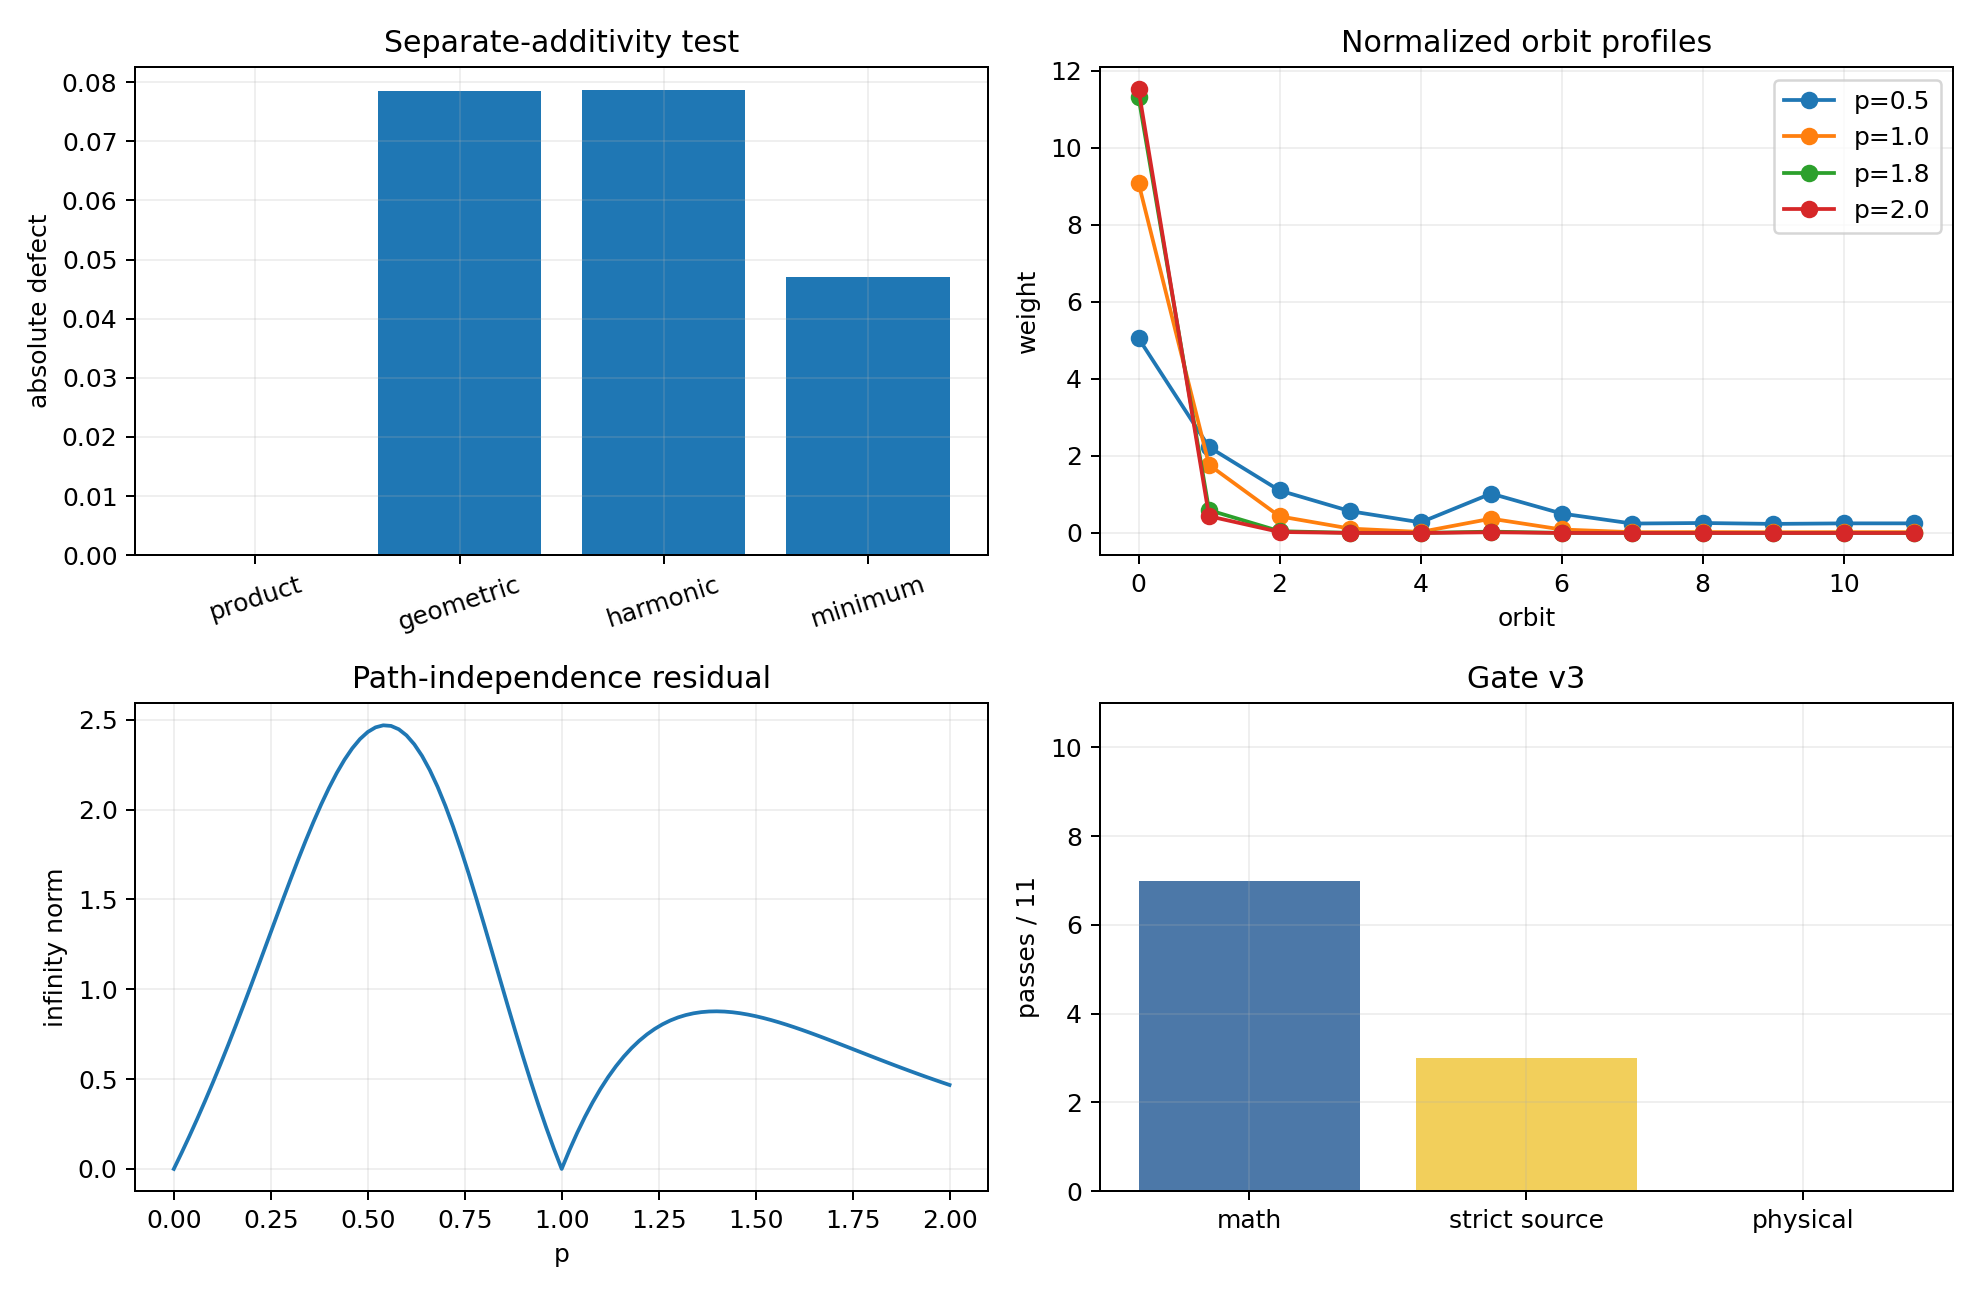
\includegraphics[width=.97\textwidth]{FIN_ST2262_ST2351_Figures/composition_refinement_and_synergy_audit.png}
\caption{Separate-additivity counterrules; normalized orbit profiles; the
identity-or-erasure residual; and gate-v3 separation of mathematical,
strict-source and physical status.}
\end{figure}

Two conditional uniqueness routes now exist:

\begin{longtable}{@{}p{.30\textwidth}p{.40\textwidth}p{.18\textwidth}@{}}
\toprule
Route & Additional premises & Result \\
\midrule\endhead
multilinear face lift & separate edge additivity + face universality &
\(\tau\) up to scale \\
fractal fixed point & multiplicativity + scale-stationary idempotence +
non-erasure & \(p=1\), identity \\
ternary state & three-body source + parity instrument + polarity &
non-Gaussian model \\
physical theory & one route + CA + local continuum + OA &
conditional only \\
\bottomrule
\end{longtable}

Neither uniqueness route is strict-derived.  The fractal route is especially
limited because its selected \(p=1\) map performs no nontrivial compression.

\subsection{Gate v3}

\[
\boxed{
7/11\ \text{mathematical constructions},\qquad
3/11\ \text{strict-source rows},\qquad
0/11\ \text{physical rows}.}
\]

The strict rows are the loop-product field, its exact \(D_{12}\) structure,
and the support-clique complex.  Separate linearity, universality,
idempotence, nontrivial refinement, irreducible ternary state, polarity,
physical scale and OA remain unsourced.

\section{Results ledger}

\begin{longtable}{@{}p{.48\textwidth}p{.25\textwidth}p{.16\textwidth}@{}}
\toprule
Statement & Status & Scope \\
\midrule\endhead
Dirichlet edge additivity forces face linearity & \status{Refuted} & category jump \\
weighted symmetry forces face universality & \status{Refuted} & Aut\(W=D_{12}\) \\
continuous multiplicative valuations are powers & \status{Proven} & positive/continuous \\
idempotence selects \(p=0,1\) & \status{Proven} & nonconstant profile \\
information preservation selects \(p=1\) & \status{Conditional} & added principle \\
\(p=1\) gives nontrivial compression & \status{Refuted} & identity map \\
nontrivial exact power self-similarity & \status{Impossible} & finite profile \\
pair instruments see hidden synergy & \status{Impossible} & zero Fisher info \\
parity is a sufficient ternary instrument & \status{Proven} & supplied model \\
strict FIN sources \(\theta\) or \(J\) & \status{Not established} & state law absent \\
fundamental physical theory follows & \status{Refuted currently} & units/OA absent \\
\bottomrule
\end{longtable}

\section{Deepest surviving interpretation}

\begin{quote}
The strict FIN pair kernel possesses a rigorous loop-product flag lift, but
neither edge composition nor its true symmetry selects a universal Hodge
valuation.  Imposing exact finite fractal self-similarity collapses the power
law to identity or erasure, so it cannot generate a nontrivial hierarchy.
Irreducible higher-order information is operationally accessible only after a
three-body state statistic and joint instrument are added.  FIN remains a
finite Dirichlet--Markov--spectral information geometry; its current pair and
refinement core cannot by itself become unique physical dynamics.
\end{quote}

\section{Next decisive direction}

The loop-function and plain-coassociativity lanes should now be frozen.
ST2352--ST2366 should test one genuinely strict non-Gaussian state law:

\begin{enumerate}[label=\textbf{ST\arabic*}, start=2352]
\item inventory strict nonlinear state laws already present in the repository;
\item test whether any contains an explicit three-body sufficient statistic;
\item compute its connected third cumulant without fitted targets;
\item test reflection covariance and nonzero polarity;
\item distinguish state source from receiver/preparation;
\item derive or reject its stationary measure;
\item test Lyapunov stability and boundedness;
\item test whether the pair kernel alone fixes its coefficient;
\item construct \(12\to24\) ternary transport;
\item test \(12\to24\to48\) path coherence;
\item test compatibility with dual unitary/diffusive channels;
\item test whether coarse records erase its signal;
\item specify the parity-level operational record;
\item audit dimensional and physical interpretation separately;
\item issue a source theorem or a no-new-live-frontier certificate.
\end{enumerate}

\section{Reproducibility and nonclaims}

Six result sets from
\texttt{FIN\_ST2262\_ST2276\_Results.json} through
\texttt{FIN\_ST2337\_ST2351\_Results.json} contain ninety packet hashes.
\texttt{test\_fin\_st2262\_st2351.py} verifies A3/A4 failures, the automorphism
theorem, normalized-power identities, the self-similarity no-go, the minimal
instrument and gate v3.

This report does not derive a strict three-body source, selector, polarity,
nontrivial fractal scale law, unique Hodge dynamics, physical units, continuum
gauge theory, apparatus, record, legacy completion, role transfer,
\(QW\)-2191, Standard Model, gravity, \(L_{\rm total}\), or Theory of
Everything.

\begin{thebibliography}{9}
\bibitem{hatcher} A. Hatcher, \emph{Algebraic Topology}, Cambridge University
Press, 2002.
\bibitem{cover} T. Cover, J. Thomas, \emph{Elements of Information Theory},
Wiley, 2006.
\bibitem{amari} S. Amari, \emph{Information Geometry and Its Applications},
Springer, 2016.
\bibitem{repo} FIN local packets and guardrails, Releases 10.76, 10.90,
11.07--11.09.
\end{thebibliography}
\end{document}
